\documentclass{article}
\usepackage{amsmath}
\usepackage{amsfonts}
\usepackage{amssymb}
\usepackage{graphicx}
\usepackage{tikz}
\usetikzlibrary{positioning,arrows.meta}

\title{LLM}
\author{Name}
\date{05/08/2025 11:13}

\begin{document}

\maketitle

\section{Building Makemore}

\subsection{Bigrams model: predict next char}
From bigrams, count the number of appearances of a pair to produce a probability distribution of the likelihood that a pair appears given the first character. We can simply draw a sample from it. One problem is that some pairs have a count of 0. When we calculate the log-likelihood, this can be an issue. We can add a "fake" count of 1.

\subsection{Neural Network approach}
We can create a training set by passing indices to tensors, encoding them using one-hot encoding. Using weights, we can project the previous character to the count table of the next character.
$$ x_{\text{encd}} \times W = \log(\text{no of counts}) $$
$$ P = \frac{C}{C.\text{Sum()}} = \text{probability of the next character} $$
We use a training sample to optimize the weights. The final result will be exactly the counting table.

\subsection{MLP}
The bigram approach can only work with a single previous character and is not extendable if we want to use more context. We can associate each word in the vocabulary with a feature vector. We can train a neural network to embed words with similar meanings into a similar space.
The proposed approach can be summarized as follows:

\begin{enumerate}
    \item Associate with each word in the vocabulary a distributed word feature vector (a real-valued vector in~$\mathbb{R}^m$). The number of features (e.g. m =30, 60 or 100 in the experiments) is much
smaller than $V$ - the size of the vocabulary (e.g. 17,000) or size of the alphabet (e.g. 26).
    \item Express the joint probability function of word sequences in terms of the feature vectors of the words in the sequence.
    \item Learn simultaneously the word feature vectors and the parameters of that probability function. 
\end{enumerate}
“Similar” words are expected to have a similar feature vector, and because the probability function is a smooth
function of these feature values, a small change in the features will induce a small change in the
probability. Therefore, the presence of only one of the above sentences in the training data will increase the probability, not only of that sentence, but also of its combinatorial number of “neighbors”
in sentence space (as represented by sequences of feature vectors).

\subsubsection{A Neural Model}
The training set is a sequence $w_1, \ldots, w_T$ of words $w_t \in V$, where the vocabulary $V$ is a large but finite set. The objective is to learn a good model 
\[
f(w_t, \ldots, w_{t - n + 1}) = \hat{P}(w_t \mid w_{1}^{t-1}).
\]
We decompose the function $f(w_t, \ldots, w_{t - n + 1}) = \hat{P}(w_t \mid w_1^{t-1})$ into two parts:
\begin{enumerate}
    \item A mapping $C$ from any element $i$ of $V$ to a real vector $C(i) \in \mathbb{R}^m$. It represents the distributed feature vectors associated with each word in the vocabulary. In practice, $C$ is represented by a $|V| \times m$ matrix of free parameters.
    
    \item The probability function over words, expressed with $C$: a function $g$ maps an input sequence of feature vectors for words in context, $(C(w_{t - n + 1}), \ldots, C(w_{t - 1}))$, to a conditional probability distribution over words in $V$ for the next word $w_t$. The output of $g$ is a vector whose $i$-th element estimates the probability $\hat{P}(w_t = i \mid w_1^{t-1})$.

    \[
    f(i, w_{t-1}, \ldots, w_{t - n + 1}) = g(i, C(w_{t - 1}), \ldots, C(w_{t - n + 1}))
    \]
\end{enumerate}

\begin{figure}\label{fig:nn_1}
    \includegraphics[scale=0.75]{nn_1.png}
    \caption{\textbf{Neural architecture:} $f(i, w_{t-1}, \ldots, w_{t - n + 1}) = g(i, C(w_{t - 1}), \ldots, C(w_{t - n + 1}))$, where $g$ is the neural network and $C(i)$ is the $i$-th word feature vector.
}
\end{figure}
The function $g$ may be implemented by a feed-forward or recurrent neural network, or another parametrized function, with parameters $\omega$. The overall parameter set is $\theta = (C, \omega)$.
Training is achieved by looking for $\theta$ that maximizes the penalized log-likelihood over the training corpus:
\[
\mathcal{L} = \frac{1}{T} \sum_{t} \log f(w_t, w_{t-1}, \ldots, w_{t - n + 1}; \theta) + R(\theta),
\]
where $R(\theta)$ is a regularization term. For example, in our experiments, $R$ is a weight decay penalty applied only to the weights of the neural network and to the $C$ matrix, not to the biases. the number of free parameters only scales linearly with V, the number of
words in the vocabulary. It also only scales linearly with the order n.

\subsubsection{Neural Network Common Issues}
\textbf{Initial Loss} is usually too high if we just start with set of random numbers. The initial loss should be based on an intial guess of the solution. For example, when predicting the next character, the initial loss should be based on the uniform probability of guressing the correct character (1/27). In theory, the weights $W_2$ should be initialized to zero, since $\log(1) = 0$, corresponding to an initial count of one for each character. However, if the final weight $W$ is set to zero, the output of the $\tanh$ layer effectively becomes the final output of the network. Consequently, computing the gradient becomes problematic, as the gradient would vanish. Recall that the backward derivative of $\tanh(t)$ is $(1 - t^2) \cdot \frac{\partial L}{\partial out}$, and the $\tanh$ activation function squeezes many values toward $-1$ and $1$, leading to zero gradients. Similar issues arise for the sigmoid and ReLU activation functions.

To avoid the \textbf{saturated tanh problem}, we can scale the weights before passing into activation function. For example, We now employ Kaiming initialization for the weights $W_1$:
$ \frac{5/3}{\sqrt{n_{in}}}. $
The gain factor of $5/3$ for the $\tanh$ activation arises from the expected value of $\tanh^2(x)$, where $x$ follows a standard Gaussian distribution:
$ \int_{-\infty}^{\infty} (\tanh x)^2 \frac{\exp(-x^2/2)}{\sqrt{2\pi}} \, dx \approx 0.39. $
The square root of this value quantifies the extent to which $\tanh$ compresses the variance of the input variable: $0.39^{0.5} \approx 0.63 \approx 3/5$. Consequently, to preserve an output variance of 1, we scale by the gain $5/3$.

However, with deep neural network, scaling all the weights become troublesome, so we can use \textbf{batch normalisation} istead. Due to the mean subtraction in batch normalization, which centers the activations, the bias term in the preceding linear layer becomes redundant and can be omitted. For a mini-batch \(\mathcal{B} = \{\mathbf{z}^{(1)}, \dots, \mathbf{z}^{(m)}\}\) of size \(m\), compute the batch mean and variance along the batch dimension:

\[
\boldsymbol{\mu}_{\mathcal{B}} = \frac{1}{m} \sum_{i=1}^{m} \mathbf{z}^{(i)},
\]

\[
\boldsymbol{\sigma}_{\mathcal{B}}^2 = \frac{1}{m} \sum_{i=1}^{m} (\mathbf{z}^{(i)} - \boldsymbol{\mu}_{\mathcal{B}})^2.
\]

The normalized pre-activation is then obtained by:

\[
\hat{\mathbf{z}}^{(i)} = \frac{\mathbf{z}^{(i)} - \boldsymbol{\mu}_{\mathcal{B}}}{\sqrt{\boldsymbol{\sigma}_{\mathcal{B}}^2 + \epsilon}},
\]

\[
\mathbf{y}^{(i)} = \boldsymbol{\gamma} \odot \hat{\mathbf{z}}^{(i)} + \boldsymbol{\beta},
\]

where \(\boldsymbol{\gamma}\) and \(\boldsymbol{\beta}\) are learnable parameters (scale and shift, respectively), \(\odot\) denotes element-wise multiplication, and \(\epsilon > 0\) is a small constant (e.g., \(10^{-5}\)) added for numerical stability to prevent division by zero when the batch variance is very small. This affine transformation allows the layer to recover the identity function if needed, preserving representational capacity.

During training, batch-specific statistics are used, but at inference time, we rely on population statistics estimated from the entire training set to enable normalization for arbitrary input sizes (e.g., single examples). These are maintained as running estimates via an exponential moving average (EMA), updated without gradient computation:

\[
\begin{aligned}
&\text{with } \texttt{torch.no\_grad()}: \\
&\quad \boldsymbol{\mu}_{\text{running}} = (1 - \tau) \cdot \boldsymbol{\mu}_{\text{running}} + \tau \cdot \boldsymbol{\mu}_{\mathcal{B}}, \\
&\quad \boldsymbol{\sigma}_{\text{running}}^2 = (1 - \tau) \cdot \boldsymbol{\sigma}_{\text{running}}^2 + \tau \cdot \boldsymbol{\sigma}_{\mathcal{B}}^2.
\end{aligned}
\]

Here, \(\tau\) is the momentum parameter set at 0.1 by default in Pytorch.

\subsubsection{Usual Plots to investigate Neural Network Performance}

To investigate common issues with Neural Network, we can use the following plots:
\begin{itemize}
    \item Loss function graph, too much volatility may imply the batch is too small
    \item Activation output distributions across layers - to check if the activation function produce extreme outputs (for example it's not good if tanh produces a lot of values close to 1,-1)
    \item Gradient distribution across different layers,  a good graph would be the gradient behaved similarly in different layers, not shrinking or exploding.
    \item Weights Gradiennt Distribtion.
    \item Gradient to Data ratio during update - a good value would be 1e-3, otherwise the update might be too slow or too fast.
\end{itemize}

\subsubsection{Quick Think on how this can be applied to financial series}


\begin{itemize}
    \item \textbf{Words are discrete:} Natural language processing benefits from a known, finite vocabulary, allowing each word to be represented as a discrete token.
    \item \textbf{Finance is continuous:} Financial data has no predefined vocabulary and can take on a continuous range of values due to its high variability and complexity.
    \item \textbf{Modeling challenge:} The absence of a discrete vocabulary in finance raises the problem of how to effectively represent continuous data in a way that supports learning and generalization.
\end{itemize}

To address
\begin{description}
    \item[Clustering techniques:] Methods like \emph{k-means}, \emph{Gaussian Mixture Models}, or \emph{Hidden Markov Models (HMMs)} can be used to group financial observations into a finite number of states or regimes.
    \item[Vector quantization:] Transforming continuous state spaces into discrete representations using quantization techniques can help bridge the gap between continuous inputs and discrete models.
    \item[Learned embeddings:] Use neural networks (e.g., autoencoders or contrastive learning) to learn compressed, structured representations of financial states that can be mapped to discrete clusters or classes.
\end{description}

\subsection{Backpropagation Example}
\subsubsection{Forward Pass}
\textbf{Variable Definitions}
\begin{itemize}
    \item $n$: Number of samples in a batch
    \item $k$: Context size (e.g., number of characters in a sequence)
    \item $m$: Number of features / embedding dimension
    \item $V$: Vocabulary size
    \item $n_1$: Number of neurons in the hidden layer
    \item $C \in \mathbb{R}^{V \times m}$: Embedding matrix
    \item $X_b \in \mathbb{R}^{n \times k}$: Input batch of character indices
    \item $Y_b \in \mathbb{R}^{n}$: Target character indices
\end{itemize}

\paragraph{Embedding Layer}
The embedding layer maps each input index to a dense vector:
\begin{align*}
    \text{emb} &= C[X_b], & \text{Shape: } \mathbb{R}^{n \times k \times m} \\
    \text{emb}_{\text{cat}} &= \text{emb.view}(n, k \times m), & \text{Shape: } \mathbb{R}^{n \times (k \cdot m)}
\end{align*}

\paragraph{Linear Layer 1}
The first hidden layer (pre-batch-normalization):
\begin{align*}
    h_{\text{prebn}} &= \text{emb}_{\text{cat}} W_1 + b_1, &
    W_1 \in \mathbb{R}^{(k \cdot m) \times n_1}, \quad b_1 \in \mathbb{R}^{1 \times n_1}, \\
    & & \text{Shape: } \mathbb{R}^{n \times n_1}
\end{align*}

\paragraph{Batch Normalization Layer}
\begin{enumerate}
    \item \textbf{Mean:}
    \begin{equation*}
        \text{bmean} = \frac{1}{n} \sum_{i=1}^{n} (h_{\text{prebn}})_i, \quad \text{Shape: } \mathbb{R}^{1 \times n_1}
    \end{equation*}

    \item \textbf{Center:}
    \begin{equation*}
        \text{bndiff} = h_{\text{prebn}} - \text{bmean}, \quad \text{Shape: } \mathbb{R}^{n \times n_1}
    \end{equation*}

    \item \textbf{Variance:}
    \begin{align*}
        \text{bndiff}^2 &= \text{bndiff} \odot \text{bndiff}, & \text{Shape: } \mathbb{R}^{n \times n_1} \\
        \text{bnvar} &= \frac{1}{n-1} \sum_{i=1}^{n} (\text{bndiff}^2)_i, & \text{Shape: } \mathbb{R}^{1 \times n_1}
    \end{align*}

    \item \textbf{Normalize:}
    \begin{align*}
        \text{bnvar\_inv} &= \frac{1}{\sqrt{\text{bnvar} + \epsilon}}, & \text{Shape: } \mathbb{R}^{1 \times n_1} \\
        \text{bnraw} &= \text{bndiff} \odot \text{bnvar\_inv}, & \text{Shape: } \mathbb{R}^{n \times n_1}
    \end{align*}

    \item \textbf{Scale and Shift:}
    \begin{equation*}
        h_{\text{preact}} = \text{bngain} \odot \text{bnraw} + \text{bnbias}, \quad \text{Shape: } \mathbb{R}^{n \times n_1}
    \end{equation*}
\end{enumerate}

\paragraph{Tanh Activation}
\begin{equation*}
    h = \tanh(h_{\text{preact}}), \quad \text{Shape: } \mathbb{R}^{n \times n_1}
\end{equation*}

\subsubsection{Output Layer \& Loss}
\begin{enumerate}
    \item \textbf{Final Linear Layer:}
    \begin{align*}
        \text{logits} &= h W_2 + b_2, &
        W_2 \in \mathbb{R}^{n_1 \times V}, \quad b_2 \in \mathbb{R}^{1 \times V}, \\
        & & \text{Shape: } \mathbb{R}^{n \times V}
    \end{align*}

    \item \textbf{Softmax (Stable):}
    \begin{align*}
        \text{logit\_maxes} &= \max_{j} (\text{logits}_{ij}), & \text{Shape: } \mathbb{R}^{n \times 1} \\
        \text{norm\_logits} &= \text{logits} - \text{logit\_maxes}, & \text{Shape: } \mathbb{R}^{n \times V} \\
        \text{counts} &= \exp(\text{norm\_logits}), & \text{Shape: } \mathbb{R}^{n \times V} \\
        \text{count\_sum} &= \sum_{j=1}^V \text{counts}_{ij}, & \text{Shape: } \mathbb{R}^{n \times 1} \\
        \text{probs} &= \frac{\text{counts}}{\text{count\_sum}}, & \text{Shape: } \mathbb{R}^{n \times V}
    \end{align*}

    \item \textbf{Cross-Entropy Loss:}
    \begin{align*}
        \text{logprobs} &= \log(\text{probs}), & \text{Shape: } \mathbb{R}^{n \times V} \\
        L &= -\frac{1}{n} \sum_{i=1}^n \text{logprobs}[i, Y_{b_i}], & \text{Scalar}
    \end{align*}
\end{enumerate}

\subsubsection{Backward Pass}

\paragraph{Gradients w.r.t. Logits}
\begin{enumerate}
    \item \textbf{$d\text{logprobs}$:}
    \begin{equation*}
        d\text{logprobs}_{ij} = 
        \begin{cases}
            -\frac{1}{n}, & j = Y_{b_i} \\
            0, & \text{otherwise}
        \end{cases}
        \quad \text{Shape: } \mathbb{R}^{n \times V}
    \end{equation*}

    \item \textbf{$d\text{probs}$:}
    \begin{equation*}
        d\text{probs} = d\text{logprobs} \odot \frac{1}{\text{probs}}, \quad \text{Shape: } \mathbb{R}^{n \times V}
    \end{equation*}

    \item \textbf{Counts and sums:}
    \begin{align*}
        d\text{count\_sum\_inv} &= \sum_{j} (d\text{probs} \odot \text{counts})_j, & \text{Shape: } \mathbb{R}^{n \times 1} \\
        d\text{count\_sum} &= d\text{count\_sum\_inv} \odot \frac{-1}{\text{count\_sum}^2}, & \mathbb{R}^{n \times 1} \\
        d\text{counts} &= d\text{probs} \odot \frac{1}{\text{count\_sum}} + d\text{count\_sum} \odot I, & \mathbb{R}^{n \times V}, I: \mathbb{R}^{n \times V}
    \end{align*}

    \item \textbf{$d\text{logits}$:}
    \begin{align*}
        d\text{norm\_logits} &= d\text{counts} \odot \exp(\text{norm\_logits}), & \mathbb{R}^{n \times V} \\
        d\text{logit\_maxes} &= \sum_{j} d\text{norm\_logits}_{ij}, & \mathbb{R}^{n \times 1} \\
        d\text{logits} &= d\text{norm\_logits} + d\text{logit\_maxes} \cdot \mathbb{I}(j = \text{argmax}_k \text{logits}_{ik}), & \mathbb{R}^{n \times V}
    \end{align*}
\end{enumerate}

\paragraph{Gradients w.r.t. Hidden Layer}
\begin{align*}
    dW_2 &= h^T d\text{logits}, & \mathbb{R}^{n_1 \times V} \\
    db_2 &= \sum_{i=1}^n (d\text{logits})_i, & \mathbb{R}^{1 \times V} \\
    dh &= d\text{logits} W_2^T, & \mathbb{R}^{n \times n_1} \\
    dh_{\text{preact}} &= dh \odot (1 - h^2), & \mathbb{R}^{n \times n_1}
\end{align*}

\paragraph{Gradients w.r.t. Batch Norm}
\begin{align*}
    d\text{bngain} &= \sum_{i=1}^n (dh_{\text{preact}} \odot \text{bnraw})_i, & \mathbb{R}^{1 \times n_1} \\
    d\text{bnbias} &= \sum_{i=1}^n (dh_{\text{preact}})_i, & \mathbb{R}^{1 \times n_1} \\
    d\text{bnraw} &= dh_{\text{preact}} \odot \text{bngain}, & \mathbb{R}^{n \times n_1} \\
    d\text{bnvar\_inv} &= \sum_{i=1}^n (d\text{bnraw} \odot \text{bndiff})_i, & \mathbb{R}^{1 \times n_1} \\
    d\text{bnvar} &= d\text{bnvar\_inv} \odot \frac{-1}{2} (\text{bnvar} + \epsilon)^{-3/2}, & \mathbb{R}^{1 \times n_1} \\
    d\text{bndiff} &= d\text{bnraw} \odot \text{bnvar\_inv} + \frac{2}{n-1} \text{bndiff} \odot d\text{bnvar}, & \mathbb{R}^{n \times n_1} \\
    dh_{\text{prebn}} &= d\text{bndiff} - \frac{1}{n} \sum_{i=1}^n (d\text{bndiff})_i, & \mathbb{R}^{n \times n_1}
\end{align*}

\paragraph{Gradients w.r.t. Embedding Layer}
\begin{align*}
    dW_1 &= \text{emb}_{\text{cat}}^T dh_{\text{prebn}}, & \mathbb{R}^{(k \cdot m) \times n_1} \\
    db_1 &= \sum_{i=1}^n (dh_{\text{prebn}})_i, & \mathbb{R}^{1 \times n_1} \\
    d\text{emb}_{\text{cat}} &= dh_{\text{prebn}} W_1^T, & \mathbb{R}^{n \times (k \cdot m)} \\
    d\text{emb} &= d\text{emb}_{\text{cat}}.\text{view}(n, k, m), & \mathbb{R}^{n \times k \times m}
\end{align*}

Finally, update $C$:
\begin{equation*}
    dC[j] \mathrel{+}= \sum_{i,l \,:\, X_{b_{il}} = j} d\text{emb}_{il}
\end{equation*}


\subsubsection{Softmax-Loss Gradient Direct calculation}

Given Loss $L = -\frac{1}{N}\sum_{i=1}^{N} \log(P_{iy_i})$ where $P_{ij} = \frac{\exp(z_{ij})}{\sum_k \exp(z_{ik})}$. We want $\frac{\partial L}{\partial z_{ij}}$.

\subsubsection*{Case 1: $j=y_i$ (derivative w.r.t. the correct logit)}
\begin{align*}
\frac{\partial}{\partial z_{iy_i}}(-\log P_{iy_i}) &= - \frac{1}{P_{iy_i}} \frac{\partial P_{iy_i}}{\partial z_{iy_i}} \\
&= - \frac{1}{P_{iy_i}} \frac{\exp(z_{iy_i})(\sum_k \exp(z_{ik})) - \exp(z_{iy_i})\exp(z_{iy_i})}{(\sum_k \exp(z_{ik}))^2} \\
&= - \frac{1}{P_{iy_i}} \left( \frac{\exp(z_{iy_i})}{\sum_k \exp(z_{ik})} - \left(\frac{\exp(z_{iy_i})}{\sum_k \exp(z_{ik})}\right)^2 \right) \\
&= - \frac{1}{P_{iy_i}} (P_{iy_i} - P_{iy_i}^2) = -(1 - P_{iy_i}) \\
&= P_{iy_i} - 1
\end{align*}

\subsubsection*{Case 2: $j \neq y_i$ (derivative w.r.t. an incorrect logit)}
\begin{align*}
\frac{\partial}{\partial z_{ij}}(-\log P_{iy_i}) &= - \frac{1}{P_{iy_i}} \frac{\partial P_{iy_i}}{\partial z_{ij}} \\
&= - \frac{1}{P_{iy_i}} \frac{-\exp(z_{iy_i})\exp(z_{ij})}{(\sum_k \exp(z_{ik}))^2} \\
&= \frac{1}{P_{iy_i}} \left( \frac{\exp(z_{iy_i})}{\sum_k \exp(z_{ik})} \cdot \frac{\exp(z_{ij})}{\sum_k \exp(z_{ik})} \right) \\
&= \frac{1}{P_{iy_i}} (P_{iy_i} \cdot P_{ij}) \\
&= P_{ij}
\end{align*}
Combining these cases (and averaging over the batch of size $n$), the gradient matrix $d\text{logits}$ is $\frac{1}{n}(P - Y)$, where $Y$ is the one-hot matrix of true labels.

\subsubsection{Batch normalisation Gradient Direct Calculation}

\begin{enumerate}
    \item \textbf{Mean ($\mu$):}
    \[
    \mu = \frac{1}{n}\sum_{i=1}^{n}x_{i}
    \]

    \item \textbf{Variance ($\sigma^2$):}
    \[
    \sigma^{2} = \frac{1}{n-1}\sum_{i=1}^{n}(x_{i}-\mu)^{2}
    \]

    \item \textbf{Normalization ($\hat{x}_i$):} The input is normalized using the batch statistics.
    \[
    \hat{x}_{i} = \frac{x_{i}-\mu}{\sqrt{\sigma^{2}+\epsilon}}
    \]

    \item \textbf{Scale and Shift ($y_i$):} The normalized activation is scaled by $\gamma$ and shifted by $\beta$.
    \[
    y_{i} = \gamma\hat{x}_{i} + \beta
    \]
\end{enumerate}

\
The goal is to compute the gradient of the loss $L$ with respect to the input of the layer, $\frac{\partial L}{\partial x_i}$. This is derived by applying the chain rule, which requires finding how the loss changes with respect to the intermediate variables $\hat{x}_i$, $\mu$, and $\sigma^2$.

First, the gradient with respect to the normalized activation $\hat{x}_i$ is found, where $\frac{\partial L}{\partial y_i}$ is the incoming gradient from the subsequent layer.
\[
\frac{\partial L}{\partial \hat{x}_{i}} = \frac{\partial L}{\partial y_{i}}\frac{\partial y_{i}}{\partial \hat{x}_{i}} = \frac{\partial L}{\partial y_{i}}\gamma
\]
Next, the gradients for the batch statistics are found by summing the contributions from all activations in the batch.
\begin{align*}
\frac{\partial L}{\partial\sigma^{2}} &= \sum_{i=1}^n \frac{\partial L}{\partial \hat{x}_{i}}\frac{\partial \hat{x}_{i}}{\partial \sigma^{2}} \\
\frac{\partial L}{\partial\mu} &= \sum_{i=1}^n \left( \frac{\partial L}{\partial \hat{x}_{i}}\frac{\partial \hat{x}_{i}}{\partial\mu} \right) + \frac{\partial L}{\partial\sigma^{2}}\frac{\partial\sigma^{2}}{\partial\mu}
\end{align*}
Finally, the total derivative for the input $x_i$ is the sum of the gradients from the three computational paths it affects: its direct path, its contribution to the mean, and its contribution to the variance.
\begin{align*}
\frac{\partial L}{\partial x_{i}} = & \quad \frac{\partial L}{\partial \hat{x}_{i}}\frac{\partial \hat{x}_{i}}{\partial x_{i}} && \text{(Path 1: Direct influence on } \hat{x}_i\text{)} \\
& + \frac{\partial L}{\partial \mu}\frac{\partial \mu}{\partial x_{i}} && \text{(Path 2: Influence via the mean)} \\
& + \frac{\partial L}{\partial\sigma^{2}}\frac{\partial \sigma^{2}}{\partial x_{i}} && \text{(Path 3: Influence via the variance)}
\end{align*}

\subsection{Simple Wavenet Implementation}
Instead of passing all the context into embedding at once, we can split the input data into small sequence length first. The idea is illustrated in \ref{fig:nn_2}.

\begin{figure}\label{fig:nn_2}
    \includegraphics[scale=0.75]{nn_2.png}
    \caption{Visualization of a stack of causal convolutional layers}.
\end{figure}


The input data will now have 3 dimensions $(N,L,C)$ where $N$ is the batch size, $L$ is the sequence length and $C$ is the number of features or channel. When doing batch normalisation, ideally we would compute the mean across the dimension (N,L). However, pyTorch batchnorm assumes the input is $(N,C,L)$ format so the mean is reduced differently.

\section{Tokenization}

Modern Large Language Models (LLMs) do not operate directly on raw text. Instead, text is converted into discrete tokens drawn from a finite vocabulary. 
Understanding this process is crucial for both interpreting model behavior and designing efficient tokenization schemes for new domains (e.g., financial data).

\subsection{From Bytes to Tokens}

GPT-style tokenization begins with a base vocabulary of 256 raw byte tokens (0--255), ensuring that \emph{any} text can be represented.
From this starting point, \textbf{Byte Pair Encoding (BPE)} merges the most frequent adjacent tokens into new tokens, gradually learning common words and subwords.

However, naive BPE can be inefficient:
\begin{itemize}
    \item It may create many variants of the same word (e.g., \texttt{dog.}, \texttt{dog!}, \texttt{dog?}), wasting vocabulary slots.
    \item Spaces, punctuation, and multi-byte characters complicate merging rules.
\end{itemize}

To address this, GPT introduces a \textbf{regex-based pre-tokenizer} before applying BPE merges.

\subsection{Regex Pre-Tokenizer Design}

The pre-tokenizer applies two key rules:
\begin{itemize}
    \item \textbf{Spaces are glued to the following word} (\verb|?\p{L}+|).  
    This avoids doubling sequence length by predicting ``space'' + word separately.  
    For example, \texttt{"dog"} and \texttt{" dog"} are treated as distinct tokens.
    
    \item \textbf{Punctuation is always split} (\verb|?[^\s\p{L}\p{N}]+|).  
    This prevents wasteful tokens like \texttt{dog.}, \texttt{dog!}, \texttt{dog?}, instead reusing \texttt{"dog"} + punctuation.
\end{itemize}

The design trade-off is:
\[
\text{spaces are extremely frequent} \;\;\to\;\; \text{glue them}, \quad
\text{punctuation is diverse and sparse} \;\;\to\;\; \text{split it}.
\]

This balances vocabulary efficiency with manageable sequence length.

\subsection{Concrete Examples}

Experiments in the notebook illustrate how different tokenizers (GPT-2 vs. GPT-4's \texttt{cl100k\_base}) handle spaces and punctuation.

\begin{center}
\begin{tabular}{|c|c|c|}
\hline
\textbf{Input Text} & \textbf{GPT-2 Tokens} & \textbf{GPT-4 Tokens} \\
\hline
\texttt{"dog."} & \texttt{["dog."]} & \texttt{["dog", "."]} \\
\texttt{"dog!"} & \texttt{["dog!"]} & \texttt{["dog", "!"]} \\
\texttt{"    hello"} & 4 separate space tokens + \texttt{"hello"} & merged into one token with spaces \\
\texttt{" world"} & \texttt{[" world"]} & \texttt{[" world"]} \\
\hline
\end{tabular}
\end{center}

Key observations:
\begin{itemize}
    \item GPT-2 leaves each space as a separate token, while GPT-4 merges consecutive spaces into a single token.
    \item Both models glue spaces to words, making \texttt{"dog"} and \texttt{" dog"} different tokens.
    \item Punctuation is separated in GPT-4, improving vocabulary efficiency.
\end{itemize}

\subsection{Beyond Text: Financial Applications}

Tokenization concepts extend beyond natural language.  
In finance, raw numbers (interest rates, prices) can be quantized or bounded:
\begin{itemize}
    \item Rates can be restricted to plausible ranges (e.g., $0$--$5\%$).  
    \item Values may be rounded to two decimal places or basis points.  
\end{itemize}

Even with such constraints, the vocabulary size may remain large, so compression techniques similar to BPE are often required.

\bigskip
In summary, tokenization is a balance between \emph{expressiveness} (capturing frequent patterns in fewer tokens) and \emph{efficiency} (avoiding unnecessary vocabulary growth). The regex pre-tokenizer in GPT demonstrates how careful design of rules for spaces and punctuation leads to practical improvements in model training and performance.


\section{Attention Mechanism and Transformer Architecture}\label{sec:Transformer}

We present the Transformer model for next-token prediction, including the core architecture and the mathematical reasoning behind several stabilisation techniques used in implementation.

\subsection{Problem Setup}
We train a character-level language model: given a context of $T$ characters, the model predicts the next token.  

\begin{itemize}
\item Vocabulary size $V$: number of unique tokens.
\item Block size $T$: context length.
\item Batch size $B$: number of sequences per batch.
\item Embedding dimension $C$: dimension of token embeddings.
\end{itemize}

The input has shape $B \times T$, mapped to embeddings of shape $B \times T \times C$.  
The model outputs logits of shape $B \times T \times V$.  

The training loss is average cross-entropy:
\[
\mathcal{L} = -\frac{1}{BT}\sum_{b=1}^B \sum_{t=1}^T \log \hat{y}_{b,t}[y_{b,t}],
\]
where $\hat{y}_{b,t} = \text{softmax}(o_{b,t})$ are predicted probabilities.

\subsection{Embeddings and Weight Tying}
Each token index $x_t$ is mapped to a vector:
\[
h_t^{(0)} = E[x_t] + P_t,
\]
with token embeddings $E \in \mathbb{R}^{V \times C}$ and positional embeddings $P_t \in \mathbb{R}^C$.  

We apply \emph{weight tying}: the same $E$ is reused for output:
\[
\text{logits}_t = h_t^{(L)} E^\top,
\]
reducing parameters and aligning input/output spaces.

\subsection{Self-Attention}
For hidden states $h \in \mathbb{R}^{T \times C}$, queries, keys, and values are
\[
Q = h W_Q, \quad K = h W_K, \quad V = h W_V,
\]
with $W_Q, W_K, W_V \in \mathbb{R}^{C \times H}$ for head size $H$.  

Attention scores:
\[
A = QK^\top.
\]

\paragraph{Scaling.}  
If $Q,K$ entries have variance 1, then $\text{Var}[QK^\top] \approx H$.  
Large $H$ yields extreme logits, saturating softmax.  
We stabilise by scaling:
\[
\tilde{A} = \frac{QK^\top}{\sqrt{H}}.
\]

\paragraph{Causal Masking.}  
To enforce autoregression:
\[
\tilde{A}_{ij} =
\begin{cases}
\frac{Q_i K_j^\top}{\sqrt{H}}, & j \leq i, \\
-\infty, & j > i,
\end{cases}
\]
so token $i$ cannot attend to the future.  
In practice, we use PyTorch’s fused scaled dot-product attention with \verb|is_causal=True|, avoiding explicit mask buffers.

\paragraph{Weighted Sum.}  
Attention weights:
\[
W = \text{softmax}(\tilde{A}),
\]
and outputs:
\[
O = W V.
\]

\subsection{Multi-Head Attention}
With $M$ heads:
\[
\text{MHA}(h) = \big[ O^{(1)} \, \| \cdots \| \, O^{(M)} \big] W_O,
\]
where $W_O \in \mathbb{R}^{MH \times C}$.  
Multiple heads allow capturing different dependency structures.

\subsection{Feedforward Network}
Each block also includes a positionwise MLP:
\[
\text{FFN}(h) = \sigma(h W_1 + b_1) W_2 + b_2,
\]
with hidden dimension $4C$ and nonlinearity $\sigma$ (GELU or ReLU).

\subsection{Residual Connections and Normalization}
Residuals:
\[
h^{(\ell+1)} = h^{(\ell)} + \frac{1}{\sqrt{2n}} f(h^{(\ell)}),
\]
where $f$ is MHA or FFN, and $n$ is the number of residual blocks.  
The scaling factor prevents residual variance from growing with depth.  

LayerNorm is applied before each sub-layer to stabilise activations.  
Unlike BatchNorm, it normalises across features within each token, making it suitable for sequences.

\subsection{Training Details and Stabilisation Tricks}

\paragraph{Initialization.}  
Linear layers are initialised as
\[
W_{ij} \sim \mathcal{N}(0, 0.02^2).
\]
Final projections are additionally scaled down by depth to avoid residual explosions.

\paragraph{Optimizer (AdamW).}  
Update rule:
\[
\theta_{t+1} = \theta_t - \eta \cdot \frac{m_t}{\sqrt{v_t} + \epsilon} - \eta \cdot \lambda \theta_t,
\]
with moving averages $m_t, v_t$ and decay coefficient $\lambda$.  
Biases and LayerNorm weights are excluded from decay for stability.

\paragraph{Learning Rate Schedule.}  
Warmup + cosine decay:
\[
\eta_t =
\begin{cases}
\eta_{\max} \cdot \frac{t}{s_w}, & t \leq s_w, \\
\eta_{\min} + \tfrac{1}{2}(\eta_{\max} - \eta_{\min})(1 + \cos \tfrac{\pi (t-s_w)}{T-s_w}), & t > s_w,
\end{cases}
\]
with warmup steps $s_w$ and total steps $T$.

\paragraph{Mixed Precision.}  
Training is run in fp16 for speed, with critical ops (softmax, LayerNorm) in fp32 to avoid numerical issues.

\paragraph{Gradient Clipping.}  
To prevent explosions:
\[
g \mapsto \frac{g}{\max(1, \|g\|_2/\tau)}, \quad \tau = 1.0.
\]

\paragraph{Validation Monitoring.}  
Data is split into train/val. Validation loss:
\[
\mathcal{L}_{\text{val}} = \frac{1}{B_{\text{val}} T}\sum_{b=1}^{B_{\text{val}}} \sum_{t=1}^T -\log \hat{y}_{b,t}[y_{b,t}],
\]
is tracked to detect overfitting.

\subsection{Summary}
The full model consists of:
\begin{enumerate}
\item Token + positional embeddings (with weight tying).
\item Stacked Transformer blocks (MHA + FFN + residuals + LayerNorm).
\item Output projection to vocabulary size.
\end{enumerate}
Stability is ensured through scaled attention, careful init, residual scaling, AdamW with selective decay, warmup+cosine scheduling, mixed precision, gradient clipping, and validation monitoring.

\begin{figure}[h]
\centering
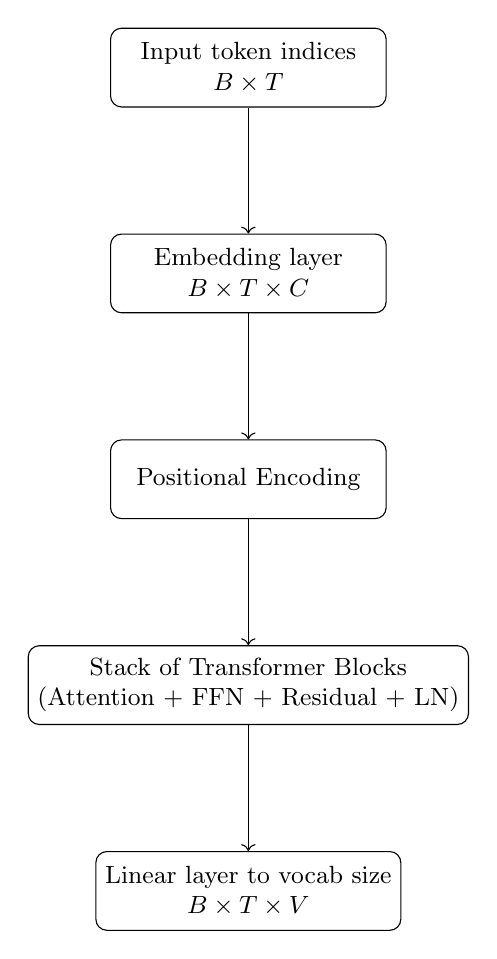
\begin{tikzpicture}[
    node distance=1.6cm,
    every node/.style={font=\small, align=center},
    box/.style={rectangle, draw, rounded corners, minimum width=3.5cm, minimum height=1cm}
]

% Input
\node[box] (input) {Input token indices \\ $B \times T$};

% Embedding
\node[box, below=of input] (embed) {Embedding layer \\ $B \times T \times C$};

% Positional Encoding
\node[box, below=of embed] (pos) {Positional Encoding};

% Transformer blocks
\node[box, below=of pos] (block) {Stack of Transformer Blocks \\ (Attention + FFN + Residual + LN)};

% Output head
\node[box, below=of block] (out) {Linear layer to vocab size \\ $B \times T \times V$};

% Arrows
\draw[->] (input) -- (embed);
\draw[->] (embed) -- (pos);
\draw[->] (pos) -- (block);
\draw[->] (block) -- (out);

\end{tikzpicture}
\caption{Flowchart of the character-level Transformer network.}
\end{figure}

\subsection{Practical Note and Link to GPT}
\begin{itemize}
    \item In practice, the tokenization is not done on character level but on sub word. Hence, the vocabulary size is typically ~10-100k tokens instead of just 65 in our problem.
    \item The context size for GPT-3 is 2048 token.
    \item After pretrainning, the base model only wants to complete documents not answering questions.
    \item The model is then fine-tunned for specific model using Reward Modeling and Reinforcement Learning.
    \item For financial application, probably a cross attention is required (encoder is for controlled variables and decoder is for the time series of variable itself)
\end{itemize}

\end{document}